\documentclass{article}

\title{Advanced Computer Graphics\\Exercise 2}
\author{Phil\'emon Favrod \and Solal Pirelli \and J\'er\'emy Rabasco}

\usepackage{amsmath}
\usepackage{tikz}
\usetikzlibrary{decorations.pathreplacing}
\usepackage{enumerate}

\begin{document}

\maketitle

\section*{Question 2.2.3}
In this answer, we will assume the following:
\begin{itemize}
\item Floating point numbers are actually considered as real numbers; and
\item \textit{drand48()} is a perfect uniform random generator in the interval $[0, 1]$.
\end{itemize}
The probability that the loop ends at a given iteration is the probability that a randomly selected point inside a cube with edges of length two is contained inside the upper hemisphere of the inscribed unit sphere. Therefore, it can be computed as
$$
\frac{V_{\text{Hemisphere}}}{V_{\text{Cube}}} = \frac{V_{\text{Sphere}}}{2V_{\text{Cube}}} = \frac{\frac{4}{3}\pi}{2^4} = \frac{\pi}{12} \approx 0.2618. 
$$

We are now wondering the expected value of a random variable following a Geometric distribution with probability of success being $p = \frac{\pi}{12}$. Therefore,
the expected number of iterations is $\frac 1p = \frac{12}{\pi} \approx 3.8197$.

\section*{Question 2.3.1}
The challenge here is to find a uniformly distributed point of the unit hemisphere given two random rel numbers uniformly distributed between 0 and 1, say $\xi_1$ and $\xi_2$. The reader might refer to Figure \ref{fig:hemisphere} to understand our solution. It basically proceeds as follows:
\begin{enumerate}[1.]
\item A rand point $r$ uniformly distributed over the circular surface which is the base of our hemisphere is generated. The methods presented in class is used here, i.e. $(\sqrt{\xi_1}, 2\pi\xi_2)$ is used instead of the naive but biased approach that takes $(\xi_2, 2\pi\xi_2)$ as a random point\footnote{The points of this sentence are represented in polar coordinates in the XY plane.}. As a reminder, the problem with the later is that points near the center of the circular surphace are more likely to be picked. %Explain more?
\item Then, this random point is projected onto the hemisphere surface by a simple application of the Pythagorean theorem resulting, in a Cartesian coordinate system, in the point
$$
p = (\sqrt{\xi_1}\cos{\left( 2\pi\xi_2\right)}, \sqrt{\xi_1}\sin{\left( 2\pi\xi_2\right)}, \sqrt{1 - \xi_1}).
$$
\end{enumerate}




\begin{figure}[h]
\centering
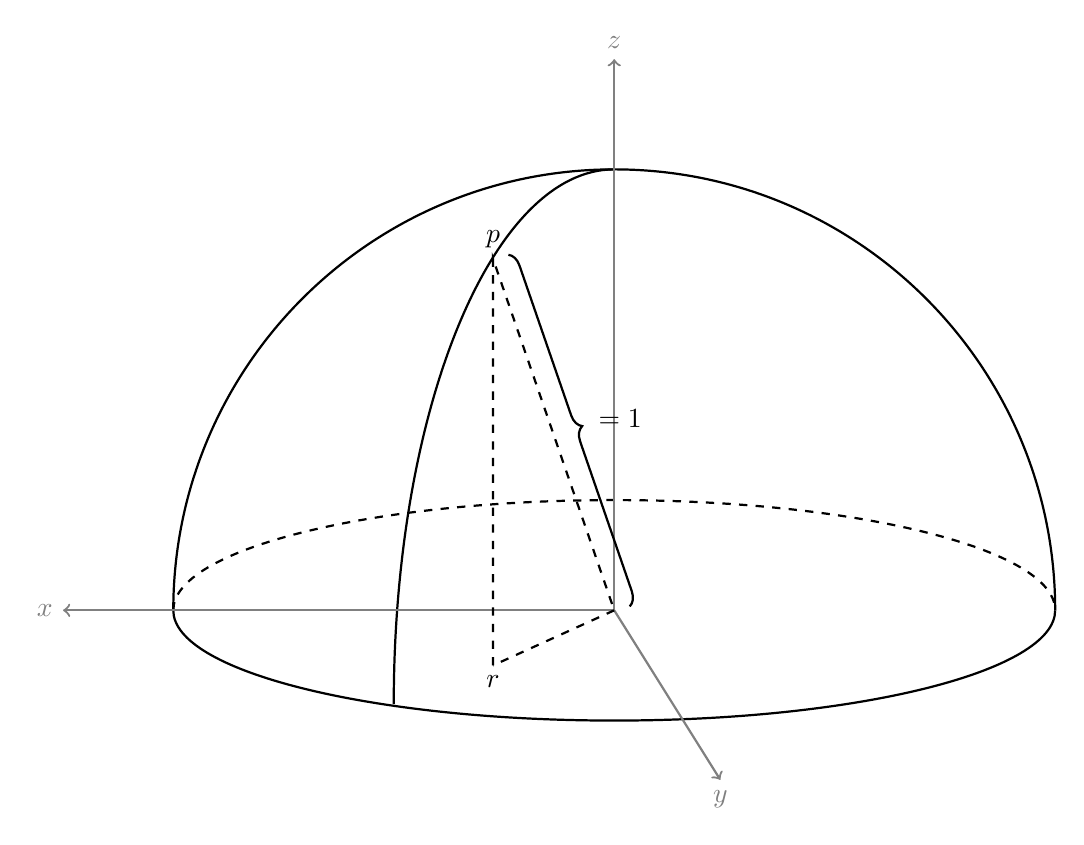
\begin{tikzpicture}[thick, scale=1.4]
% base circle
\draw (0,0) arc (180:360:4 and 1);
\draw [dashed] (0,0) arc (180:0:4 and 1);

% hemisphere
\draw (0,0) arc (180:0:4 and 4);
\draw (2,-.85) arc (180:90:2 and 4.85);

% axes
\draw [->, gray] (4,0,0) -- ++(-5,0,0)node[anchor=east]{$x$};
\draw [->, gray] (4,0,0) -- ++(0,-2.5,-2.5)node[anchor=north]{$y$};
\draw [<-, gray] (4,5)node[anchor=south]{$z$} -- (4, 0);

% schema
\draw [dashed] (4,0) -- (2.9,-0.5)node[anchor=north] {$r$};
\draw [dashed] (2.9, -0.5) -- (2.9, 3.19)node[anchor=south] {$p$} -- (4,0);
\draw [decorate,decoration={brace,amplitude=5pt},xshift=4pt,yshift=1pt]
(2.9, 3.19) -- (4,0) node [black,midway,xshift=0.65cm, yshift=0.15cm]{$= 1$};
\end{tikzpicture}
\caption{Generating a uniformly distributed random point of a unit hemisphere given two uniformly distributed random real numbers between 0 and 1.}
\label{fig:hemisphere}
\end{figure}

\end{document}